\documentclass[aspectratio=43]{beamer}
\usepackage[T1]{fontenc}

%\documentclass[aspectratio=169]{beamer}
\usetheme{Madrid} % My favorite!
%\usetheme{Boadilla} % Pretty neat, soft color.
%\usetheme{default}
%\usetheme{Warsaw}
%\usetheme{Bergen} % This template has nagivation on the left
%\usetheme{Frankfurt} % Similar to the default 
%\usetheme{Copenhagen}
%\usetheme{Goettingen}
%\usetheme{Ilmenau}
%with an extra region at the top.
%\usecolortheme{seahorse} % Simple and clean template
%\usetheme{Darmstadt} % not so good
% Uncomment the following line if you want %
% page numbers and using Warsaw theme%
% \setbeamertemplate{footline}[page number]
%\setbeamercovered{transparent}
\setbeamercovered{invisible}
\setbeamersize{text margin right=3.5mm, text margin left=7.5mm}  % text margin
\setbeamertemplate{caption}[numbered]

\setbeamerfont{page number in head/foot}{size=\large}
\setbeamertemplate{footline}[frame number]


% To remove the navigation symbols from 
% the bottom of slides%

\usepackage{graphicx}
\usepackage{epstopdf}
\usepackage{booktabs}
\usepackage{array}
\usepackage{adjustbox}


\renewcommand{\arraystretch}{1.3}
\usepackage{rotating}
\usepackage{pifont}
\usepackage{hyperref}
\usepackage{fontawesome}
\usepackage[list=false, listformat=simple]{subcaption}
\captionsetup{compatibility=false}

\pdfstringdefDisableCommands{
\let\\\space
}



\usepackage{amsmath,amsfonts,amsthm,color,psfrag,epsf, tabularx, multirow, longtable, pdflscape}

\usepackage{tikz}
\usetikzlibrary{shapes,shapes.misc,arrows,positioning,calc,fit}

\usepackage{pgfplots}
\pgfplotsset{compat=1.13}
\usepackage{tikz}
\usepackage{appendixnumberbeamer}
\usepackage{csquotes}


\usepackage[detect-weight=true, binary-units=true, range-units=single]{siunitx} % Properly Centered numbers in tables

\usetikzlibrary{shapes, graphs, quotes, arrows, backgrounds, positioning, calc}
\usepackage{calc}

\usepackage[
backend=biber,
autocite=superscript,
natbib=true,
style=authoryear,
sorting=none]{biblatex}
\AtEveryCitekey{\clearfield{url}}

\addbibresource{Thesis.bib}
\addbibresource{Post-Thesis.bib}


\usepackage{pifont}
\newcommand*\OK{\ding{51}} % requires pifont


\usepackage{amsmath,amsthm, amssymb, latexsym}
\usepackage{booktabs}
\usepackage{colortbl}
\usepackage{hyperref}
%\usepackage[textsize=tiny]{todonotes}
%\presetkeys{todonotes}{inline}{}

\interdisplaylinepenalty=2500
\hyphenpenalty=10000

\usepackage[english]{babel}
\addto\captionsenglish{\renewcommand{\figurename}{Fig.}}

\def\checkmark{\tikz\fill[scale=0.4](0,.35) -- (.25,0) -- (1,.7) -- (.25,.15) -- cycle;} 
\def\scalecheck{\resizebox{\widthof{\checkmark}*\ratio{\widthof{x}}{\widthof{\normalsize x}}}{!}{\checkmark}}
%that's defined it - now for a test



\makeatletter
\newcommand*{\minuscellcolor}{}
\def\minuscellcolor\ignorespaces{%
% \ignorespaces not really needed, because \@ifnextchar gobbles spaces
\pgfdeclareshape{roundedNode}{
	\inheritsavedanchors[from=rectangle] % this is nearly a rectangle
	\inheritanchorborder[from=rectangle]
	\inheritanchor[from=rectangle]{center}
	\inheritanchor[from=rectangle]{north}
	\inheritanchor[from=rectangle]{south}
	\inheritanchor[from=rectangle]{west}
	\inheritanchor[from=rectangle]{east}
	\backgroundpath{% this is new
		% store lower right in xa/ya and upper right in xb/yb
		\southwest \pgf@xa=\pgf@x \pgf@ya=\pgf@y
		\northeast \pgf@xb=\pgf@x \pgf@yb=\pgf@y
		% construct main path
		\pgfsetcornersarced{\pgfpoint{5pt}{5pt}}
		\pgfpathmoveto{\pgfpoint{\pgf@xa}{\pgf@ya}}
		\pgfpathlineto{\pgfpoint{\pgf@xa}{\pgf@yb}}
		\pgfpathlineto{\pgfpoint{\pgf@xb}{\pgf@yb}}
		\pgfsetcornersarced{\pgfpoint{5pt}{5pt}}
		\pgfpathlineto{\pgfpoint{\pgf@xb}{\pgf@ya}}
		\pgfpathclose
	}
}
%http://tex.stackexchange.com/questions/89166/centering-in-tabularx-and-x-columns
\newcolumntype{Y}{>{\centering\arraybackslash}X}

% http://tex.stackexchange.com/questions/98388/how-to-make-table-with-rotated-table-headers-in-latex
\newcommand*\rot{\rotatebox{90}}
\newcommand*\OK{\ding{51}} % requires pifont

\@ifnextchar-{\cellcolor[HTML]{FFAAAA}}{}
}
\newcolumntype{L}{>{\minuscellcolor}l}
\newcolumntype{C}{>{\minuscellcolor}c}
\newcolumntype{R}{>{\minuscellcolor}r}
\makeatother
%http://tex.stackexchange.com/questions/132783/how-to-write-checkmark-in-latex
\def\checkmark{\tikz\fill[scale=0.4](0,.35) -- (.25,0) -- (1,.7) -- (.25,.15) -- cycle;} 

\tikzset{
	block/.style = {draw, fill=white, rectangle, minimum height=3em, minimum width=3em, text width=8em, text centered},
	tmp/.style  = {coordinate}, 
	sum/.style= {draw, fill=white, circle, node distance=1cm},
	input/.style = {coordinate},
	output/.style= {coordinate},
	pinstyle/.style = {pin edge={to-,thin,black}
	},
	from/.style args={#1 to #2}{% without transformations
		above right={0cm of #1},% needs positioning library
		/utils/exec=\pgfpointdiff
		{\tikz@scan@one@point\pgfutil@firstofone(#1)\relax}
		{\tikz@scan@one@point\pgfutil@firstofone(#2)\relax},
		minimum width/.expanded=\the\pgf@x,
		minimum height/.expanded=\the\pgf@y},
	doc/.style={draw, shape=roundedNode, align=center},
	bluefill/.style={fill=blue, opacity=0.5, text opacity=1}
}
\tikzset{
	*|/.style={
		to path={
			(perpendicular cs: horizontal line through={(\tikztostart)},
			vertical line through={(\tikztotarget)})
			% is the same as (\tikztostart -| \tikztotarget)
			% but just to be safe: http://tex.stackexchange.com/a/29781/16595
			-- (\tikztotarget) \tikztonodes
		}
	}
}

% USAGE: \cercle {center} {radius in cm} {begin degrees} {value of the arc} {line width} {color}
% \coordinate (OO) at (2.8,2.2);
% \cercle{OO}{0.5cm}{-20}{60}{1.0pt}{blue};
\newcommand{\cercle}[6]{
	\node[circle,inner sep=0,minimum size={2*#2}](a) at (#1) {};
	\draw[#6,line width=#5] (a.#3) arc (#3:{#3+#4}:#2);
}


% \SpecialCoor
\def\subsum{\mathit{\Sigma}}

\newcommand*\rot{\rotatebox{90}}
\tikzset{
block/.style = {draw, fill=white, rectangle, minimum height=3em, minimum width=3em, text width=8em, text centered},
tmp/.style  = {coordinate}, 
sum/.style= {draw, fill=white, circle, node distance=1cm},
input/.style = {coordinate},
output/.style= {coordinate},
pinstyle/.style = {pin edge={to-,thin,black}
},
from/.style args={#1 to #2}{% without transformations
above right={0cm of #1},% needs positioning library
/utils/exec=\pgfpointdiff
{\tikz@scan@one@point\pgfutil@firstofone(#1)\relax}
{\tikz@scan@one@point\pgfutil@firstofone(#2)\relax},
minimum width/.expanded=\the\pgf@x,
minimum height/.expanded=\the\pgf@y},
doc/.style={draw, shape=roundedNode, align=center},
bluefill/.style={fill=blue, opacity=0.5, text opacity=1}
}
\tikzset{
*|/.style={
to path={
(perpendicular cs: horizontal line through={(\tikztostart)},
vertical line through={(\tikztotarget)})
% is the same as (\tikztostart -| \tikztotarget)
% but just to be safe: http://tex.stackexchange.com/a/29781/16595
-- (\tikztotarget) \tikztonodes
}
}
}
\graphicspath{{../Figures/}{../posters/PDW-15/figures/},{./img/}}
\DeclareGraphicsExtensions{.pdf,.png,.jpg}
%\usepackage{bm}         % For typesetting bold math (not \mathbold)
%\logo{\includegraphics[height=0.6cm]{yourlogo.eps}}


%

% If you have a file called "university-logo-filename.xxx", where xxx
% is a graphic format that can be processed by latex or pdflatex,
% resp., then you can add a logo as follows:

\pgfdeclareimage[height=0.5cm]{university-logo}{img/livuni}
\logo{\pgfuseimage{university-logo}}



% Delete this, if you do not want the table of contents to pop up at
% the beginning of each subsection:
\AtBeginSubsection[]
{
\begin{frame}<beamer>{Outline}
  \tableofcontents[currentsection,currentsubsection]
\end{frame}
}


\begin{document}

\title{An Investigation into Trust and Reputation Frameworks for Autonomous Underwater Vehicles}

\author{\begin{tabular}{r@{ }l} 
  Author:      & Andrew Bolster \\[1ex] 
  Supervisors: & Prof. Alan Marshall, Prof. Simon Maskell (UoL)\\
               & Prof. Jean-Guy Fontaine (UPMC)
             \end{tabular}}
\institute[UoL]{University of Liverpool}
\date[06/10/16]{Thursday 6th October 2016}
% \today will show current date. 
% Alternatively, you can specify a date.
\begin{frame}
  \titlepage
\end{frame}

\frame{\tableofcontents}
\section{Structure}

\begin{frame}{Structure of this presentation}
	\begin{block}{Structure}
		\begin{itemize}
			\item Statement of Research Purpose
			\item Summary of Contributions
			\item Errata
			\item Discussion of new research that has entered the field since submission
			\item Chapter Summaries
			\item Open for Discussion
		\end{itemize}
	\end{block}
	% TODO
\end{frame}

\section{Contributions, Errata \& State of the Field}

\begin{frame}{Summary of Contributions}
	\begin{columns}
		\begin{column}{0.45\textwidth}
			\begin{exampleblock}{Primary}
				\begin{itemize}
					\item Trust in UANs
					\item Trust assessment based on Physical Behaviours
					\item Multi-domain Trust 
				\end{itemize}
			\end{exampleblock}
			\begin{block}{Secondary}
				\begin{itemize}
					\item Automatic weighting of MTFM
					\item Agent based UAN Sim
					\item Synthetic Domains from metrics over multiple domains
					\item Review of Trust in the marine defence context
				\end{itemize}
			\end{block}
		\end{column}
		\begin{column}{0.56\textwidth}
			\begin{block}{Publications}
				\begin{itemize}  
					\item Analytical Metric Weight Generation for Multi-Domain Trust in Autonomous Underwater MANETs. IEEE UComms 2016
					\item Single \& Multi-metric Trust Management Frameworks for Use in Underwater Autonomous Networks. IEEE TrustCom 2015
					\item Analysis of Trust Interfaces in Autonomous \& Semi-Autonomous Collaborative MHPC Operations, The Technical Cooperation Program, Portsmouth, UK 2014.
					\item A Multi-Vector Trust Framework for Autonomous Systems, AAAI 2014.
				\end{itemize}  
			\end{block}
		\end{column}
	\end{columns}
\end{frame}

\begin{frame}{Erratta}
	\begin{alertblock}{Erratta}
		\begin{itemize}
			\item Many small typographic issues corrected
			\item Missing Citation in 3.1.1,5-7 \footfullcite{Urick1983}
			\item Out-of-order paragraphs in 4.2.5 (Top should be bottom)
		\end{itemize}
	\end{alertblock}
	
\end{frame}

\begin{frame}{Recent Research Trends}
	\begin{block}{Trust}
		\begin{itemize}
			\item Interesting general move towards decentralised trust \footcite{Korzun2015}
			\item Ditto cohort based relative trust assessment \footcite{Singh2016}
			\item Increasing use of ML techniques to assess contextual trust dynamically \footcite{Rishwaraj2017} 
			\item Human Factors emerging as a increasingly vital area of research \footcite{Saeidi2009,Matthews2016,Lahijanian2016}
			\item Novel/Updated techniques for generalised TMF assessment are emerging \footcite{Janiszewski2016} 
		\end{itemize}
	\end{block}
	
\end{frame}

\begin{frame}{Recent Research Trends}
	\begin{block}{Acomms} %most cites from ucomms
		\begin{itemize}
			\item Assumptions of Gaussian noise naive for real applications \footcite{Mahmood2016, Deane2016}
			\item The Beaufort Sea has fundamentally changed it's characteristics in 20 years and highlights fundamental flaws in channel modelling assumptions \footcite{Schmidt2016}
			\item Higher-Stack level functionality problems remain open( i.e. MAC+Route+ID+Interop) \footcite{Diamant2016,Petroccia2016,Petroccia2016a, Anjangi2016}
			\item Assumptions on increasing accuracy and timeliness of passive localisation proving accurate \footcite{Vio2016, Ferreira2016,Das2016}
		\end{itemize}
	\end{block}
	
\end{frame}

\section{Chapter Summaries}

\begin{frame}{Chapter 1: Introduction}

  \begin{columns}
    \begin{column}{0.5\textwidth}
      \begin{block}{Focus On}
        \begin{itemize}
          \item Trust
          \item Autonomy
          \item Decentralised networks
          \item Harsh Environments
        \end{itemize}
      \end{block}
    \end{column}
    \begin{column}{0.5\textwidth}
      \begin{alertblock}{Stated deficiencies in}
        \begin{itemize}
          \item Single Metric Trust
          \item Threats from Capable actors
          \item Systemic Trust
          \item Lack of modelling of Trust in Harsh environments
        \end{itemize}
      \end{alertblock}
    \end{column}
  \end{columns}
\end{frame}

\begin{frame}{Chapter 2: MANETs and Trust} 
    \begin{columns}
    	\begin{column}{0.5\textwidth}
			\begin{block}{Focus On}
				\begin{itemize}
					\item Network/Graph concepts
					\item Routing
					\item Trust Perspectives and Models
					\item Trust Relationships
					\item Multi-Party Trust
					\item Trusted Threats
					\item Autonomy and Design constraints of Autonomous Systems
					\item Current Trust Management Frameworks
				\end{itemize}
			\end{block}
    	\end{column}
    	\begin{column}{0.5\textwidth}
    		\begin{exampleblock}{Key Outcomes}
    			\begin{itemize}
    				\item Definition of Trust
    				\item Levels \& Constraints of Autonomy
    	            \item Lack Specification and Validation for Autonomous Systems
    				\item Threats to Trust
    				\item Threats to MANETs
    				\item Need for Trust in Autonomous Systems

    			\end{itemize}
    		\end{exampleblock}
    	\end{column}
    \end{columns}
      
\end{frame}

\begin{frame}{Chapter 3: Maritime Communications and Operations}
      \begin{columns}
		\begin{column}{0.5\textwidth}
			\begin{block}{Focus On}
				\begin{itemize}
					\item Marine Acoustics
					\item AComms Modelling 
					\item AUV Operations
					\item Need for Trust in AUV AComms
				\end{itemize}
			\end{block}
		\end{column}
		\begin{column}{0.5\textwidth}
			\begin{exampleblock}{Key Outcomes}
				\begin{itemize}
					\item Channel Emulation Models
					\item Selection of characteristic constraints
					\item Threat Surface
					\item Operational / Kinematic constraints and Scenario selection
				\end{itemize}
			\end{exampleblock}
		\end{column}
      \end{columns}
      
\end{frame}

\begin{frame}{Chapter 4: Assessment of TMF Performance in Marine Environments}
  \begin{columns}
    \begin{column}{0.5\textwidth}
      \begin{block}{Focus On}
        \begin{itemize}
          \item Comparative factors between UAN/WLAN
	      \item Relevant Metric Selection re AComms
          \item Comparison of Single \& Multi Metric TMFs in UAN
          \item MTFM weight variation assessment and regression
        \end{itemize}
      \end{block}
    \end{column}
    \begin{column}{0.5\textwidth}
      \begin{exampleblock}{Key Findings}
        \begin{itemize}
          \item Modelled optimal performance range @ $\approx$0.015-0.025pps/100-300m node separations \hyperlink{fig:2d_normed_product}{\beamergotobutton{Details}}
          \item MTFM outperforms single metric TMFs for selected misbehaviours \hyperlink{fig:otmf_beta_comparison_boxes}{\beamergotobutton{Details}}
          \item MTFM vector weighting further improves performance and tolerance \hyperlink{fig:all_mobile_badmouthing}{\beamergotobutton{Details}}
          \item Long collection times due to sparsity can impact trust assessment relevance

        \end{itemize}
      \end{exampleblock}
    \end{column}
  \end{columns}

\end{frame}
\begin{frame}{Chapter 5: Use of Physical Behaviours for Trust Assessment}
  \begin{columns}
    \begin{column}{0.5\textwidth}
      \begin{block}{Focus On}
        \begin{itemize}
          \item Physical Misbehaviours and Metrics
          \item ``Failure'' vs ``Selfish'' vs ``Malice''
          \item AUV Kinematics
          \item Metric variability in collaborative collision avoidance (flocking)
          \item Metric based classifier
        \end{itemize}
      \end{block}
    \end{column}
    \begin{column}{0.5\textwidth}
      \begin{exampleblock}{Key Findings}
        \begin{itemize}
        	\item First physical misbehaviour detection system in UAN
        	\item Demonstrated that different misbehaviours impact different physical metrics differently \hyperlink{fig:metric_values}{\beamergotobutton{Details 1}} \hyperlink{fig:summedsigmabar}{\beamergotobutton{Details 2}}
        	\item Highly accurate, manually configured, blind behaviour classifier ($\approx$ 0\% FP, $\gtrapprox$ 90 \% TP)
        \end{itemize}
      \end{exampleblock}
    \end{column}
  \end{columns}
\end{frame}

\begin{frame}{Chapter 6: Multi-Domain Trust Assessment in Collaborative Marine MANETs}
	\begin{columns}
		\begin{column}{0.5\textwidth}
			\begin{block}{Focus On}
				\begin{itemize}
					\item Combination of comms. \& phys. metrics
					\item Random Forest based metric significance correlation to build $H$ weighting vector for MTFM
					\item Domain specific behaviour effects across domain space
					\item Relative vector weight measurement across cohort ($\Delta T, \Delta T^-$)
					\item Generation and Appraisal of alternate/targeted ``domains''
				\end{itemize}
			\end{block}
		\end{column}
		\begin{column}{0.5\textwidth}
			\begin{exampleblock}{Key Findings}
				\begin{itemize}
					\item Misbehaviours impact across domains (not obvious) \hyperlink{fig:alternate_domain_diag}{\beamergotobutton{Details}}
					\item Inherent redundancy (eg INDD/$P_{RX}$) allows differential behaviours to be detected \hyperlink{fig:positive_heat}{\beamergotobutton{Details}}
					\item Application level selfishness (STS) very difficult to automatically 
					\item Extended Ch4 behaviour based optimisation of MTFM to dynamically select most significant metrics
				\end{itemize}
			\end{exampleblock}
		\end{column}
	\end{columns}
\end{frame}



\section*{Summary of Contributions to the Field}

\begin{frame}{Summary of Contributions to the Field}
  % Keep the summary *very short*.
	\begin{block}{$\Sigma$}
		\begin{itemize}
			\item UWA Multi Metric/Domain Trust
			\item UWA Trust is \alert{Hard} \& it's mostly the channels' fault
			\item Discrimination of non-comms misbehaviours/failures \structure{even just using comms metrics}
			\item Methodology for exploring / training / metric relevance
			\item Single-Metric Trust is \alert{unstable} in such an environments
			\item Multi-Metric Trust works \& can \alert{discriminate behaviours}
			\item \alert{Not all metrics} are equally useful
			\item Simple classifiers \alert{can} be very good in \alert{some} behaviours (MPC)
			\item - can be \alert{not so good} for others (STS)
		\end{itemize}
	\end{block}
\end{frame}

\begin{frame}{Outstanding Research Challenges}
  \begin{alertblock}{$\notin$}
    \begin{itemize}
      \item Smarter Detection Classifier
      \item Cooperative / Periodic / Variable attack profiles
      \item Further assessment of impact and tolerance of misbehaviours in the network
      \item Commonality of detection filters across Multiple-base scenarios
      \item \alert{Real} experiments and Cross validation implementations
      \item Heterogenous Node capabilities / Mixed-mission characteristics
      \item Extension to logical routing domain
      \item Application of mixed-domain trust assessment to non-physical systems
      \item Reflective Trust (i.e. systems trust of the operator)

    \end{itemize}
  \end{alertblock}
\end{frame}

\begin{frame}[t,allowframebreaks]
  \frametitle{References}
  
  \printbibliography[title=References]% [nottype=video]}
\end{frame}

\appendix

\section{Chapter 1}

\begin{frame}{Fig 1.1 Multi-Domain Threat Surface}
	\begin{figure}[h!]
		\centering
		\includegraphics[width=1.1\linewidth]{threat_surface_sum}
		\caption[Multi-Domain Threat Surface]{Multi-Domain Threat Surface}
		\label{fig:threat_surface}
	\end{figure}
\end{frame}

\section{Chapter 2}

\begin{frame}{Tab 2.3 Definitions of Trust}
\begin{table}[h]
	\centering
	\label{tab:trust_definitions}
	\adjustbox{max height=\dimexpr\textheight -4.2cm\relax,
		max width=\textwidth}{
	\begin{tabularx}{\textwidth}{X p{2.2cm}}\toprule
		Definition & Source \\ \midrule
		Assured reliance on the character, ability, strength, or truth of someone or something.
		& Merriam-Webster\\
		Firm belief in the reliability, truth, or ability of someone or something & OED\\
		The willingness of a party to be vulnerable to the actions of another party based on the expectation that the other will perform a articular action important to the trustor, irrespective of the ability to monitor or control that other party &~\citet{Mayer1995} \\
		An expectancy held by and individual or a group that the word, promise, verbal or written statement of another individual or group can be relied upon &~\citet{Rotter1967}\\\bottomrule
	\end{tabularx}}
\end{table}
\end{frame}

\begin{frame}{Fig 2.5 Model of Trust}
\begin{figure}[h]
	\centering
			\adjustbox{max height=\dimexpr\textheight -2.2cm\relax,
				max width=\textwidth}{
	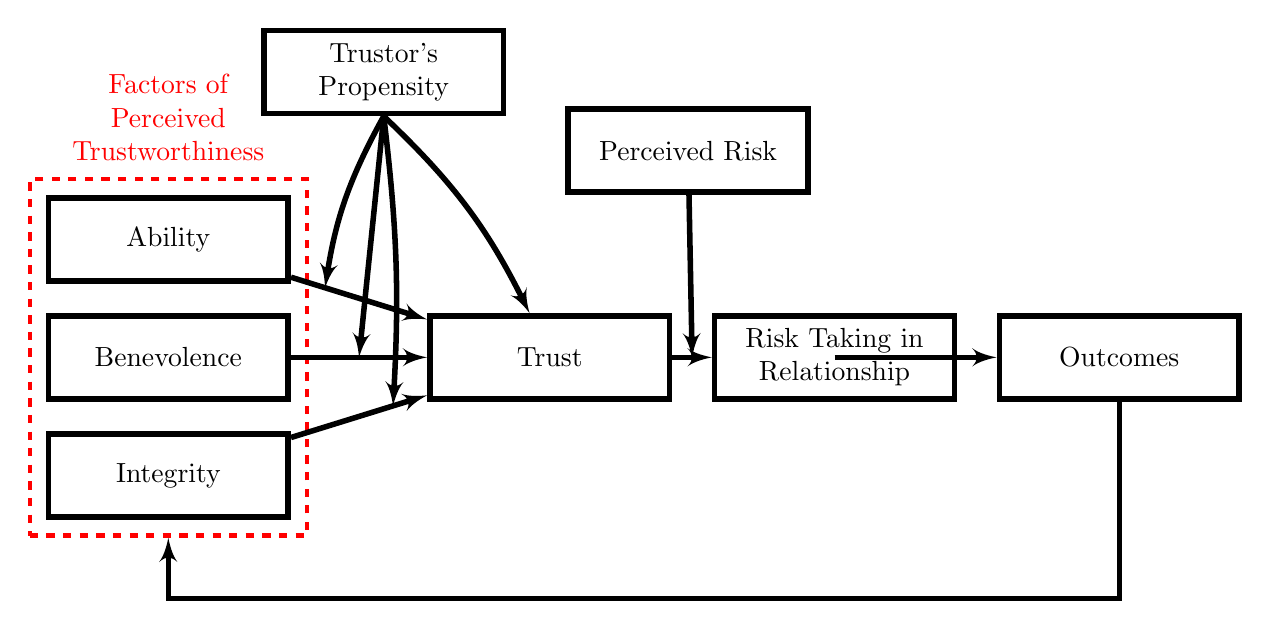
\begin{tikzpicture}[auto, node distance=1.5cm and 0.5cm, line width=2pt, >=latex']
	\node [block] (ability) {Ability};
	\node [block, below of = ability] (benevolence) {Benevolence};
	\node [block, below of = benevolence] (integrity) {Integrity};
	%\draw[red,thick,dotted] ($(ability.north west)+(-0.3,0.6)$)  rectangle ($(integrity.south east)+(0.3,-0.6)$);
	\node (percievedFactors) [draw=red, fit= (ability) (benevolence) (integrity), inner sep=0.2cm, dashed, ultra thick, fill opacity=0.2] {};
	\node [yshift=5ex, red, text width=8em, text centered] at (percievedFactors.north) {Factors of Perceived Trustworthiness};
	
	\node [block, right=1.5cm and 1.5cm of percievedFactors] (trust) {Trust};
	
	\node [block, above=2.5cm of trust, xshift=-6em] (trustorsPropensity) {Trustor's Propensity};
	\node [block, right=of trust] (riskTaking) {Risk Taking in Relationship};
	\node [block, above=of trust, xshift=5em] (percievedRisk) {Perceived Risk};
	\node [block, right=of riskTaking] (outcomes) {Outcomes};
	
	\draw [->] (ability) --coordinate[near start](mAb)  (trust);
	\draw [->] (benevolence) -- coordinate[midway](mBe) (trust);
	\draw [->] (integrity) -- coordinate[near end](mIn) (trust);
	\draw [->] (trustorsPropensity.south) to[bend right=10] (mAb);
	\draw [->] (trustorsPropensity.south) to (mBe);
	\draw [->] (trustorsPropensity.south) to[bend left=5] (mIn);
	\draw [->] (trustorsPropensity.south) to[bend left=10] (trust);
	\draw [->] (trust) -- coordinate[midway](mT) (riskTaking);
	\draw [->] (percievedRisk) -- (mT);
	\draw [->] (riskTaking) |- (outcomes);
	\draw [->] (outcomes.south) --++ (0cm,-2.5cm) -| (percievedFactors.south);
	
	\end{tikzpicture}}
	\caption[Model of Trust]{Model of Trust (from~\citet{Mayer1995})}
	\label{fig:mayer_trust_model}
\end{figure}
\end{frame}

\begin{frame}{Fig 2.6 Trust Construct Relationships}
	\begin{figure}
		\centering
		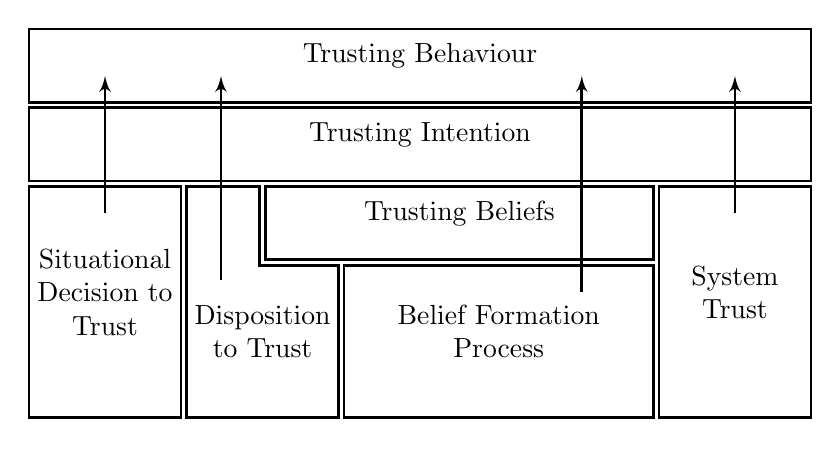
\begin{tikzpicture}[auto, node distance=1.5cm and 0.5cm, line width=1pt, >=latex', every node/.style = {align=center, minimum height=1em}]
		\node[fit={(0,0)(2,3)}, draw=black, inner sep=-1pt] (sit) {Situational Decision to Trust};
		
		\node[fit={(2,0)(4,2)}] (disp) {Disposition to Trust};
		\path[draw=black] (2cm+1pt,0cm+1pt) -- (4cm-1pt,0cm+1pt) -- (4cm-1pt,2cm-1pt) -- (3cm-1pt,2cm-1pt) -- (3cm-1pt,3cm-1pt) -- (2cm+1pt,3cm-1pt) -- cycle;
		
		\node[fit={(4,0)(8,2)}, draw=black, inner sep=-1pt] (belief) {Belief Formation\\Process};
		\node[fit={(8,0)(10,3)}, draw=black, inner sep=-1pt] (sys) {System\\Trust};
		
		\node[fit={(3,2)(8,3)}, draw=black, inner sep=-1pt] (trustb) {Trusting Beliefs};
		\node[fit={(0,3)(10,4)}, draw=black, inner sep=-1pt] (trusti) {Trusting Intention};
		\node[fit={(0,4)(10,5)}, draw=black, inner sep=-1pt] (trusth) {Trusting Behaviour};
		
		
		\draw[<-, *|] ([yshift=10pt]trusth.south) to ([yshift=-10pt]sit.north);
		\draw[<-, *|] ([yshift=10pt]trusth.south) to ([yshift=-10pt, xshift=-15pt]disp.north);	
		\draw[<-, *|] ([yshift=10pt]trusth.south) to ([yshift=-10pt, xshift=30pt]belief.north);
		\draw[<-, *|] ([yshift=10pt]trusth.south) to ([yshift=-10pt]sys.north);	
		
		
		\end{tikzpicture}
		\caption[Trust Construct Relationships]{Trust Construct Relationships (from~\citet{Liu2010})}
		\label{fig:trust_constructs}
	\end{figure}
\end{frame}


\begin{frame}{Fig 2.10 Trust Topologies}
	
	\begin{figure}
		\centering
		
		\begin{subfigure}[t]{0.24\textwidth}
			\adjustbox{max height=\dimexpr\textheight-5.5cm\relax,
				max width=\textwidth}{
			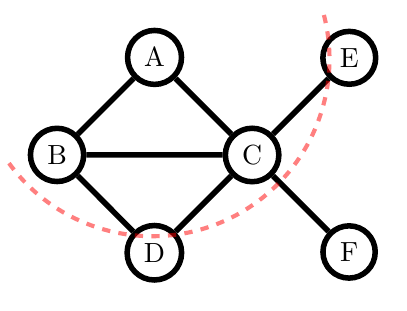
\begin{tikzpicture}[auto, node distance=1.5cm and 0.5cm, line width=2pt, >=latex']
			\node [sum, preaction={fill=red!20}] (a) {A};
			\node [sum, below left =of a] (b) {B};
			\node [sum, below right =of a] (c) {C};
			\node [sum, below left =of c] (d) {D};
			\node [sum, above right =of c] (e) {E};
			\node [sum, below right =of c] (f) {F};
			
			\graph{
				(a) -- (b);
				(a) -- (c);
				(b) -- (c);
				(b) -- (d);
				(c) -- (d);
				(c) -- (e);
				(c) -- (f);
			};
			
			\begin{pgfinterruptboundingbox}
			\coordinate (A) at (a);
			\cercle{A}{2.25cm}{216}{160}{1.50}{red, opacity=0.5, dashed};
			\end{pgfinterruptboundingbox}
			\end{tikzpicture}}
			\caption{Topology}
		\end{subfigure}
		\hfill
		\begin{subfigure}[t]{0.25\textwidth}
			\adjustbox{max height=\dimexpr\textheight-5.5cm\relax,
				max width=\textwidth}{
			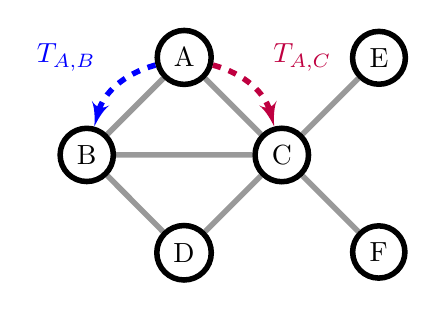
\begin{tikzpicture}[auto, node distance=1.5cm and 0.5cm, line width=2pt, >=latex']
			\node [sum, preaction={fill=red!20}] (a) {A};
			\node [sum, below left =of a] (b) {B};
			\node [sum, below right =of a] (c) {C};
			\node [sum, below left =of c] (d) {D};
			\node [sum, above right =of c] (e) {E};
			\node [sum, below right =of c] (f) {F};
			
			
			\graph[edges={opacity=0.4}]{
				(a) -- (b);
				(a) -- (c);
				(b) -- (c);
				(b) -- (d);
				(c) -- (d);
				(c) -- (e);
				(c) -- (f);
			};
			
			\draw[->, blue, dashed] (a) to[bend right] (b) node [left of=a] {$T_{A,B}$};
			\draw[->, purple, dashed] (a) to[bend left] (c) node [right of=a] {$T_{A,C}$};
			
			\end{tikzpicture}}
			\caption{Direct}
		\end{subfigure}
		\hfill
		\begin{subfigure}[t]{0.24\textwidth}
			\adjustbox{max height=\dimexpr\textheight-5.5cm\relax,
				max width=\textwidth}{
			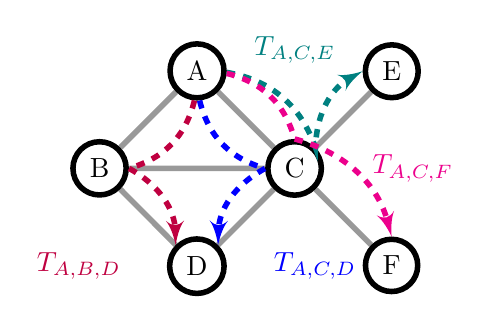
\begin{tikzpicture}[auto, node distance=1.5cm and 0.5cm, line width=2pt, >=latex']
			\node [sum, preaction={fill=red!20}] (a) {A};
			\node [sum, below left =of a] (b) {B};
			\node [sum, below right =of a] (c) {C};
			\node [sum, below left =of c] (d) {D};
			\node [sum, above right =of c] (e) {E};
			\node [sum, below right =of c] (f) {F};
			
			
			\graph[edges={opacity=0.4}]{
				(a) -- (b);
				(a) -- (c);
				(b) -- (c);
				(b) -- (d);
				(c) -- (d);
				(c) -- (e);
				(c) -- (f);
			};
			
			\draw[->, blue, dashed] (a) to[bend right] (c.west) to [bend right](d.north east) node [right of=d] {$T_{A,C,D}$};
			\draw[->, purple, dashed] (a) to[bend left] (b.east) to [bend left](d.north west) node [left of=d] {$T_{A,B,D}$};
			\draw[->, teal, dashed] (a) to[bend left] (c.north east) to [bend left](e.west) node [above of=c] {$T_{A,C,E}$};
			\draw[->, magenta, dashed] (a) to[bend left] (c.north) to [bend left](f.north) node [right of=c] {$T_{A,C,F}$};
			\end{tikzpicture}}
			\caption{Indirect}
			
		\end{subfigure}
		\hfill
		\begin{subfigure}[t]{0.24\textwidth}
			\adjustbox{max height=\dimexpr\textheight-5.5cm\relax,
				max width=\textwidth}{
			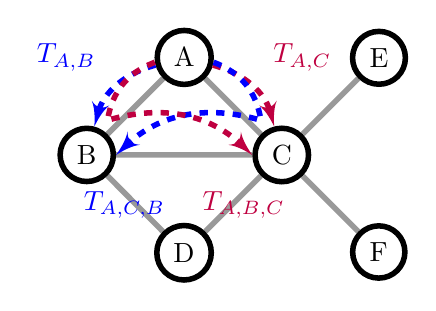
\begin{tikzpicture}[auto, node distance=1.5cm and 0.5cm, line width=2pt, >=latex']
			\node [sum, preaction={fill=red!20}] (a) {A};
			\node [sum, below left =of a] (b) {B};
			\node [sum, below right =of a] (c) {C};
			\node [sum, below left =of c] (d) {D};
			\node [sum, above right =of c] (e) {E};
			\node [sum, below right =of c] (f) {F};
			
			
			\graph[edges={opacity=0.4}]{
				(a) -- (b);
				(a) -- (c);
				(b) -- (c);
				(b) -- (d);
				(c) -- (d);
				(c) -- (e);
				(c) -- (f);
			};
			
			\draw[->, blue, dashed] (a) to[bend right] (b) node [left of=a] {$T_{A,B}$};
			\draw[->, purple, dashed] (a) to[bend left] (c) node [right of=a] {$T_{A,C}$};
			
			\draw[->, blue, dashed] (a) to[bend left] ([yshift=5pt] c.north west) to [bend right](b.east)  node [above left of=d, xshift=2ex, yshift=-3ex] {$T_{A,C,B}$} ;
			\draw[->, purple, dashed] (a) to[bend right] ([yshift=5pt] b.north east) to [bend left](c.west) node [above right of=d, xshift=-2ex, yshift=-3ex] {$T_{A,B,C}$};
			
			\end{tikzpicture}}
			\caption{Recommender}
			
		\end{subfigure}
		\hfill
		\caption{Trust Topologies; Direct, Indirect, Recommender, etc.\ from the perspective of Node A}
		\label{fig:trust_topology_relationships}
	\end{figure}
\end{frame}

\section{Chapter 3}

\begin{frame}{Fig 3.3: Bellhop Model}
	
	\begin{figure}
		\begin{subfigure}[t]{0.3\textwidth}
			\centering
			\includegraphics[width=\textwidth]{ssp_linear_increasing}
			\caption{Linear Increasing}
			\label{fig:ssp_linear_increasing}
		\end{subfigure}
		\begin{subfigure}[t]{0.3\textwidth}
			\centering
			\includegraphics[width=\textwidth]{ssp_linear_decreasing}
			\caption{Linear Decreasing}
			\label{fig:ssp_linear_decreasing}
		\end{subfigure}
		
		\begin{subfigure}[t]{0.3\textwidth}
			\centering
			\includegraphics[width=\textwidth]{ssp_n_squared}
			\caption{Quadratic}
			\label{fig:ssp_n_squared}
		\end{subfigure}
		\begin{subfigure}[t]{0.3\textwidth}
			\centering
			\includegraphics[width=\textwidth]{ssp_isovelocity}
			\caption{Isovelocity}
			\label{fig:ssp_isovelocity}
		\end{subfigure}
		\caption{Bellhop Model of Non-Linear Marine Shortest-Path Propagation in various Speed of Sound Profiles}
		\label{fig:ssps}
	\end{figure}
\end{frame}




\begin{frame}{Communications Channel Considerations}
  Key Characteristics of the Marine Acoustic Channel \cite{Urick1983,Partan2006,Stojanovic2007,Stefanov2011}:
  \begin{itemize}
    \item Slow propagation ($~1400ms^{-1}$) incurring long delays
    \item Inter-symbol interference
    \item Doppler Spreading
    \item Non-Linear propagation due to refraction
    \item Fast \& Slow fades from environmental factors (flora/fauna/surface and seabed conditions)
    \item Freq. dependant attenuation
    \item Significant destructive multipath effects
  \end{itemize}

\end{frame}

\begin{frame}{Attenuation in the Marine Acoustic Channel}

  The attenuation that occurs in an underwater acoustic channel over distance $d$ about frequency $f$ is given as $A_{\text{aco}}(d,f) = A_0d^ka(f)^d$ or
  %
  \begin{equation}
    \label{eq:acoattenuationdb}
    10 \log A_{\text{aco}}(d,f)/A_0 = k \cdot 10 \log d + d \cdot 10 \log a(f)
  \end{equation}
  %
  where $A_0$ is a normalising constant, $k$ is a spreading factor, and $a(f)$ is the absorption coefficient\cite{Stefanov2011};
  %
  \begin{equation}
    \label{eq:thorp}
    10 \log a(f) = \frac{0.11 \cdot f^2}{1+f^2} + \frac{44\cdot f^2}{4100+f^2}+ 2.75\times10^{-4} f^2 + 0.003
  \end{equation}

  \pause

  Compared to RF Free space PL: $(A_{\text{RF}}(d,f) \approx \left( \frac{4\pi d f}{c} \right)^2)$
  \begin{itemize}
    \item \alert{Exponential} in $d$: $A_{\text{aco}} \propto f^{d}$ vs $A_{\text{RF}} \propto (df)^2$
    \item $f$ factor \alert{four orders higher} in $f\propto A_{\text{aco}}$ vs $f\propto A_{\text{RF}}$

  \end{itemize}

\end{frame}

\begin{frame}{Multi-Metric TMF - Grey Grading} 
  \begin{equation}
    \label{eq:grcg}
    \theta_{k,j}^t = \frac{\min_k|a_{k,j}^t - g_j^t| + \rho \max_k|a_{k,j}^t-g_j^t|}{|a_{k,j}^t-g_j^t| + \rho \max_k|a_{k,j}^t-g_j^t|} 
  \end{equation}
  \begin{equation}
    \label{eq:grcb}
    \phi_{k,j}^t = \frac{\min_k|a_{k,j}^t - b_j^t| + \rho \max_k|a_{k,j}^t-b_j^t|}{|a_{k,j}^t-b_j^t| + \rho \max_k|a_{k,j}^t-b_j^t|} 
  \end{equation}
  \begin{equation}
    \label{eq:grc}
    [\theta_k^t, \phi_k^t] = \left[\sum_{j=0}^M h_j \theta_{k,j}^t,\sum_{j=0}^M h_j \phi_{k,j}^t \right]
  \end{equation}
  \begin{equation}
    \label{eq:grcT}
    T_k^t = ({1+{(\phi_k^t)^2}/{(\theta_k^t)^2}})^{-1}
  \end{equation}

  Where  $a_{k,j}^t$ is the value of an observed metric $x_j$ for a given node $k$ at time $t$,  $g$ and $b$ are respectively the ``good'' and ``bad'' reference metric sequences from $\{a_{k,j}^t k=1,2\dots K\}$, $H=[h_0\dots h_M]$ is a metric weighting vector such that $\sum h_j = 1$

\end{frame}
\begin{frame}{Multi-Metric TMF - Topological Relationships} 
  \centering
  Includes shared assessments from other nodes weighted based on their relative topology to provide a final value\footnotemark  

  \vspace{9pt}

  $T_{i,j}^{MTFM}$
  \begin{figure}[h]
    \centering
    \includegraphics[height=.65\textheight]{node_relationships}
    \label{fig:node_relationships}
  \end{figure}

\end{frame}


\begin{frame}[allowframebreaks]{Grey Trust Equs}
  \begin{align}
    \label{eq:networkeffects}
    T_{i,j}^{MTFM}=&\frac{1}{2} \cdot \max_s\{f_s(T_{i,j})\} T_{i,j}\\ \notag
    +&\frac{1}{2} \frac{2|N_R| }{2|N_R| + |N_I|}\sum_{n \in N_R} \max_s\{f_s(T_{i,n})\} T_{i,n}\\ \notag
    +&\frac{1}{2} \frac{|N_I| }{2|N_R| + |N_I|}\sum_{n \in N_I} \max_s\{f_s(T_{i,n})\} T_{i,n} 
  \end{align}

  Where $T_{i,n}$ is the subjective trust assessment of $n_i$ by $n_n$, and $f_s = [ f_1,f_2, f_3]$ given as...

  \framebreak

  \begin{align}
    \label{eq:whitenization}
    f_1(x)&= -x+1\notag\\
    f_2(x)&= 
    \begin{cases}
      2x & \text{if }x\leq 0.5\\
      -2x+2 & \text{if }x>0.5
    \end{cases}\\
    f_3(x)&= x\notag
  \end{align}
  \hyperlink{fig:node_relationships}{\beamergotobutton{Back}}
\end{frame}


\begin{frame}{Tab 4.1: System Model Constraints}
  \centering
  \begin{table}[h]
      \label{tab:sysconstraints}
	    \adjustbox{max height=\dimexpr\textheight-5cm\relax,
	    	max width=\textwidth}{%
      \begin{tabular}{lccc}
        \toprule
        Parameter & Unit & Terrestrial & Marine \\
        \midrule
        Simulated Duration & $s$ & 300 & 18000\\
        Trust Sampling Period & $s$ & 1 & 600 \\
        Simulated Area & $km^2$ & 0.7 & 0.7-4 \\
        Transmission Range & $km$ & 0.25 & 1.5 \\
        Physical Layer & & RF(802.11) & Acoustic\\
        Propagation Speed& $m/s$ & $3\times10^8$ & 1490\\
        Center Frequency& $Hz$ & $2.6\times10^9$ & $2 \times 10^4$ \\
        Bandwidth& $Hz$ & $22\times10^6$ & $1\times10^4$\\
        MAC Type & & CSMA/DCF & CSMA/CA\\
        Routing Protocol & & DSDV & FBR \\
        Max Speed & $ms^{-1}$ & 5 & 1.5 \\
        Max Data Rate & $bps$ & $5\times10^6$ & $\approx 240$ \\
        Packet Size & bits & 4096 &  9600 \\
        Single Transmission Duration & $s$ & 10 & 32 \\
        Single Transmission Size & bits & $10^7$ & $9600$ \\
        \bottomrule
      \end{tabular}}
  \end{table}
\end{frame}
\section{Chapter 4}
\begin{frame}{Throughput}
	\begin{figure}[h]
		\begin{subfigure}[t]{0.3\textwidth}
			\centering
			\includegraphics[width=\textwidth]{throughput_2d_bella_static}
			\caption{Static}
			\label{fig:throughput_2d_bella_static}
		\end{subfigure}
		\begin{subfigure}[t]{0.3\textwidth}
			\centering
			\includegraphics[width=\textwidth]{throughput_2d_bella_single_mobile}
			\caption{Single Mobile}
			\label{fig:throughput_2d_bella_single_mobile}
		\end{subfigure}
		
		\begin{subfigure}[t]{0.3\textwidth}
			\centering
			\includegraphics[width=\textwidth]{throughput_2d_bella_allbut1_mobile}
			\caption{All-but-one Mobile}
			\label{fig:throughput_2d_bella_allbut1_mobile}
		\end{subfigure}
		\begin{subfigure}[t]{0.3\textwidth}
			\centering
			\includegraphics[width=\textwidth]{throughput_2d_bella_all_mobile}
			\caption{All Mobile}
			\label{fig:throughput_2d_bella_all_mobile}
		\end{subfigure}
		\label{fig:2d_throughput}
	\end{figure}
\end{frame}

\begin{frame}{Delay}
	\begin{figure}[h]
		\begin{subfigure}[t]{0.3\textwidth}
			\centering
			\includegraphics[width=\textwidth]{delay_2d_bella_static}
			\caption{Static}
			\label{fig:delay_2d_bella_static}
		\end{subfigure}
		\begin{subfigure}[t]{0.3\textwidth}
			\centering
			\includegraphics[width=\textwidth]{delay_2d_bella_single_mobile}
			\caption{Single Mobile}
			\label{fig:delay_2d_bella_single_mobile}
		\end{subfigure}
		
		\begin{subfigure}[t]{0.3\textwidth}
			\centering
			\includegraphics[width=\textwidth]{delay_2d_bella_allbut1_mobile}
			\caption{All-but-one Mobile}
			\label{fig:delay_2d_bella_allbut1_mobile}
		\end{subfigure}
		\begin{subfigure}[t]{0.3\textwidth}
			\centering
			\includegraphics[width=\textwidth]{delay_2d_bella_all_mobile}
			\caption{All Mobile}
			\label{fig:delay_2d_bella_all_mobile}
		\end{subfigure}
		\label{fig:2d_delay}
	\end{figure}
\end{frame}

\begin{frame}{Fig 4.12: Normalised Throughput-Delay Product}
	\begin{figure}[h]
		\begin{subfigure}[t]{0.3\textwidth}
			\centering
			\includegraphics[width=\textwidth]{2d_normed_product_bella_static}
			\caption{Static}
			\label{fig:2d_normed_product_bella_static}
		\end{subfigure}
		\begin{subfigure}[t]{0.3\textwidth}
			\centering
			\includegraphics[width=\textwidth]{2d_normed_product_bella_single_mobile}
			\caption{Single Mobile}
			\label{fig:2d_normed_product_bella_single_mobile}
		\end{subfigure}
		
		\begin{subfigure}[t]{0.3\textwidth}
			\centering
			\includegraphics[width=\textwidth]{2d_normed_product_bella_allbut1_mobile}
			\caption{All-but-one Mobile}
			\label{fig:2d_normed_product_bella_allbut1_mobile}
		\end{subfigure}
		\begin{subfigure}[t]{0.3\textwidth}
			\centering
			\includegraphics[width=\textwidth]{2d_normed_product_bella_all_mobile}
			\caption{All Mobile}
			\label{fig:2d_normed_product_bella_all_mobile}
		\end{subfigure}
		\label{fig:2d_normed_product}
	\end{figure}
\end{frame}


\begin{frame}{Fig 4.14: Hermes, OTMF, MTFM Trust assessments}
	\begin{figure}[t]
		\centering

			\begin{subfigure}{0.3\textwidth}	
				\includegraphics[width=\linewidth]{trust_beta_otmf_fair}
				\caption{Fair Scenario}
				\label{fig:all_mobile_fair_beta}
			\end{subfigure}
			\begin{subfigure}{0.3\textwidth}
				\includegraphics[width=\linewidth]{trust_beta_otmf_malicious} 
				\caption{Malicious Power Control (MPC) Scenario}
				\label{fig:all_mobile_badmouthing_beta}
			\end{subfigure} 
			\begin{subfigure}{0.3\textwidth}	
				\includegraphics[width=\linewidth]{trust_beta_otmf_selfish} 
				\caption{Selfish Target Selection (STS) Scenario}
				\label{fig:all_mobile_selfish_beta}
			\end{subfigure}

		\caption{$T_{0,1}$ for Hermes, OTMF, MTFM assessment values for fair and malicious behaviours in the fully mobile scenario}
		\label{fig:otmf_beta_comparison}
	\end{figure}
\end{frame}
\begin{frame}{Fig. 4.15: Alternate Assessment Visualisation}
	\begin{figure}
		\centering
		\includegraphics[width=0.8\textwidth]{trust_beta_otmf_mtfm_boxes}
		\caption{Visualisation of TMF performance comparison across Fair, MPC and STS scenarios}
		\label{fig:otmf_beta_comparison_boxes}
	\end{figure}
\end{frame}

\begin{frame}
	\begin{figure}[h]
		\centering
		\begin{subfigure}{0.3\textwidth}
			\includegraphics[width=\linewidth]{trust_bella_all_mobile_emph_ADelay_BadMouthingPowerControl} 
			\caption{$\text{Delay}$ Emphasised}
			\label{fig:all_mobile_badmouthing_delay}
		\end{subfigure}
		\begin{subfigure}{0.3\textwidth}
			\includegraphics[width=\linewidth]{trust_bella_all_mobile_emph_PLR_BadMouthingPowerControl} 
			\caption{$PLR$ Emphasised}
			\label{fig:all_mobile_badmouthing_plr}
		\end{subfigure}
		\begin{subfigure}{0.3\textwidth}
			\includegraphics[width=\linewidth]{trust_bella_all_mobile_emph_ARXP_BadMouthingPowerControl} 
			\caption{Received Power ($P_{RX}$) Emphasised}
			\label{fig:all_mobile_badmouthing_rxp}
		\end{subfigure}	
		\begin{subfigure}{0.3\textwidth}
			\includegraphics[width=\linewidth]{trust_bella_all_mobile_emph_ATXP_BadMouthingPowerControl} 
			\caption{Transmit Power ($P_{TX}$) Emphasised}
			\label{fig:all_mobile_badmouthing_txp}
		\end{subfigure}
		\begin{subfigure}{0.3\textwidth}
			\includegraphics[width=\linewidth]{trust_bella_all_mobile_emph_RXThroughput_BadMouthingPowerControl} 
			\caption{Throughput ($S$) Emphasised}
			\label{fig:all_mobile_badmouthing_rxthroughput}
		\end{subfigure}
		\begin{subfigure}{0.3\textwidth}
			\includegraphics[width=\linewidth]{trust_bella_all_mobile_emph_TXThroughput_BadMouthingPowerControl} 
			\caption{Offered Load ($G$) Emphasised}
			\label{fig:all_mobile_badmouthing_txthroughput}
		\end{subfigure}
		\caption{$T_{1,0}^\text{MTFM}$ in the All Mobile case for the Malicious Power Control behaviour}
		\label{fig:all_mobile_badmouthing}
	\end{figure}
\end{frame}

\begin{frame}{Fig 4.18: Factor Analysis}
	\begin{figure}
		\centering
		\includegraphics[height=0.78\textheight]{MaliciousSelfishMetricFactors}
		\caption{Random Forest Factor Analysis of Malicious, Selfish and Fair behaviours compared against each-other}
		\label{fig:malselfactors}
	\end{figure}
\end{frame}


\section{Chapter 5}

\begin{frame}{Fig 5.3: Observed Metric Values}
	\begin{figure}
		\centering
		\includegraphics[height=0.9\textheight]{Metric_Values}
		\label{fig:metric_values}
	\end{figure}
\end{frame}
\begin{frame}{Fig 5.4: Relative Node Deviance}
	\begin{figure}
		\centering
		\includegraphics[width=\linewidth]{summedsigmabar}
		\caption{Per-Node-Per-Run deviance for each metric, normalised in time ($\sum\alpha/T$)}
		\label{fig:summedsigmabar}
	\end{figure}
\end{frame}


\section{Chapter 6}
\begin{frame}{Fig 6.1: Alternate Domain Construction}
	\begin{figure}[h]
		\centering
		  \adjustbox{max height=\dimexpr\textheight -2.2cm\relax,
		  	max width=\textwidth}{
		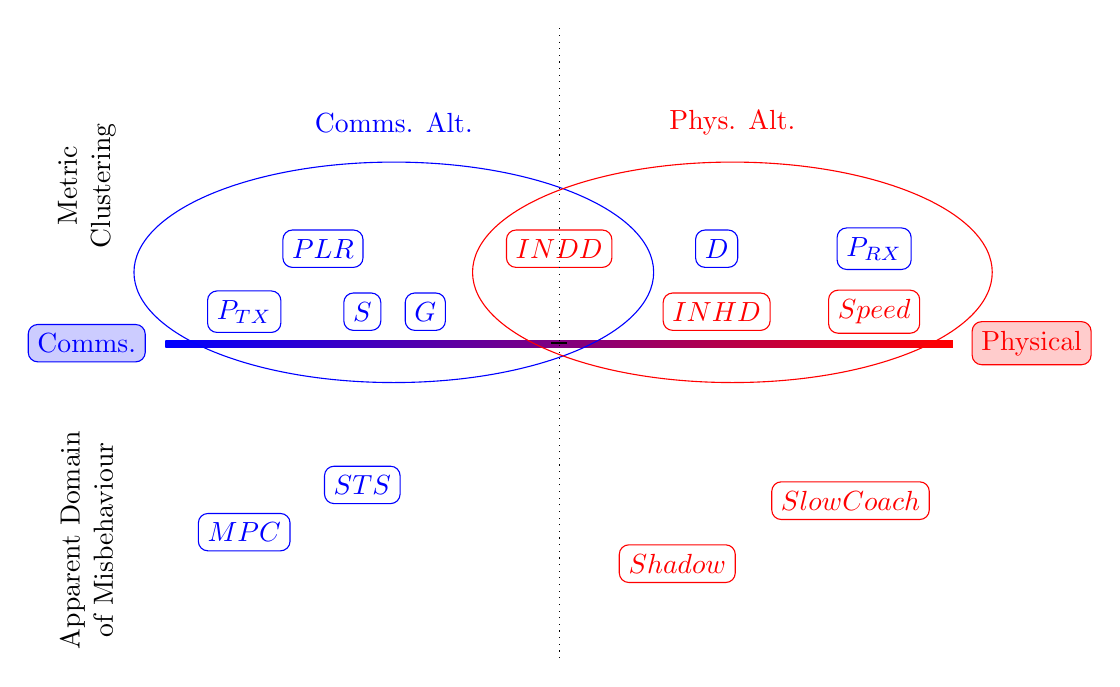
\begin{tikzpicture}[-latex,
		comms/.style={text=blue, draw=blue, rounded corners=.8ex},
		phys/.style={text=red, draw=red, rounded corners=.8ex}]
		% Start off with the line
		%\draw [<-|][comms, draw=blue, very thick] (0,1) -- (5,1); 
		%\draw [|->][phys, draw=red, very thick] (5,1) -- (10,1); 
		\path[left color=blue,right color=red]
		(0,0.95) rectangle +(10,2.5pt);
		
		% Baseline labels
		\node[comms, fill=blue, fill opacity=0.2, text opacity=1] at (-1,1) {Comms.};
		\node[phys, fill=red, fill opacity=0.2, text opacity=1] at (11,1) {Physical};
		
		% Metric Labels
		\node[comms] at (7,2.2) {$D$};
		\node[comms] at (9,2.2) {$P_{RX}$};
		\node[comms] at (1,1.4) {$P_{TX}$};
		\node[comms] at (2.5,1.4) {$S$};
		\node[comms] at (3.3,1.4) {$G$};
		\node[comms] at (2,2.2) {$PLR$};
		\node[phys] at (5,2.2) {$INDD$};
		\node[phys] at (7,1.4) {$INHD$};
		\node[phys] at (9,1.4) {$Speed$};
		
		\node[rotate=90, align=center] at (-1, 3) {Metric\\Clustering};
		\node[rotate=90, align=center] at (-1, -1.5) {Apparent Domain\\of Misbehaviour};
		\node[comms] at (1,-1.4) {$MPC$};
		\node[comms] at (2.5,-0.8) {$STS$};
		\node[phys] at (6.5,-1.8) {$Shadow$};
		\node[phys] at (8.7,-1) {$SlowCoach$};
		
		% Draw approx subsets
		\draw[comms] (2.9,1.9) ellipse (3.3 and 1.4);
		\draw[phys] (7.2,1.9) ellipse (3.3 and 1.4);
		
		\node[text=red] at (7.2,3.8) {Phys. Alt.};
		\node[text=blue] at (2.9,3.8) {Comms. Alt.};
		
		% Misc
		\draw[-|][dotted] (5,5) -- (5,1);
		\draw[-|][dotted] (5,-3) -- (5,1);
		
		
		\end{tikzpicture}}
		\caption{Assumptions made about the relevant domains of impact / detectability of misbehaviours, and domain relevance of metrics, may not be optimal}
		\label{fig:alternate_domain_diag}
	\end{figure}
\end{frame}


\begin{frame}{Fig 6.2: Communications Metric Features}

\begin{figure}[h!]
	\centering

	\includegraphics[height=\dimexpr\textheight -2.2cm\relax]{comms_metric_trust_relevance}
	\caption{Communications Metric Features ($X_{comms}$)}
	\label{fig:comms_feature_extraction}
\end{figure}
\end{frame}
\begin{frame}{Fig 6.3: Physical Metric Features}
	
\begin{figure}[h!]
	\centering
	\includegraphics[height=\dimexpr\textheight -2.2cm\relax]{phys_metric_trust_relevance}
	\caption{Physical Metric Features ($X_{phys}$)}
	\label{fig:phys_feature_extraction}
\end{figure}
\end{frame}
\begin{frame}{Fig 6.4: Multi Domain  Metric Features}
	
\begin{figure}[h!]
	\centering
	\includegraphics[height=\dimexpr\textheight -2.2cm\relax]{full_metric_trust_relevance}
	\caption{Multi Domain  Metric Features ($X_{merge}$)}
	\label{fig:multi_feature_extraction}
\end{figure}
\end{frame}
\begin{frame}{Tab 6.1: Multi Domain Metric Feature Correlation}
	
\begin{table}
	\centering
	\caption{Multi Domain Metric Feature Correlation ($X_{merge}$)}
			  \adjustbox{max height=\dimexpr\textheight -2.2cm\relax,
			  	max width=\textwidth}{
	\begin{tabular}{lrrrrrrrrr}
\toprule
{} &  $Delay$ &  $P_{RX}$ &  $P_{TX}$ &  $T^P_{RX}$ &  $PLR$ &  $T^P_{TX}$ &  $INDD$ &  $INHD$ &  $Speed$ \\
Misbehaviour &          &           &           &             &        &             &         &         &          \\
\midrule
MPC          &   -0.187 &     0.129 &     0.579 &       0.006 &  0.069 &      -0.146 &   0.040 &  -0.190 &   -0.297 \\
STS          &   -0.195 &    -0.035 &     0.019 &      -0.100 &  0.019 &       0.381 &  -0.209 &   0.057 &    0.062 \\
Shadow       &    0.004 &    -0.654 &     0.030 &      -0.016 &  0.030 &       0.063 &   0.120 &   0.158 &    0.266 \\
SlowCoach    &   -0.157 &    -0.533 &     0.013 &      -0.132 &  0.013 &      -0.028 &   0.159 &   0.206 &    0.460 \\
\bottomrule
\end{tabular}
}
	\label{tab:full_metric_correlations}
\end{table}
\end{frame}

\begin{frame}{Fig 6.10: Accuracy Characteristics}
	\begin{figure}
		\centering
		\includegraphics[width=\linewidth]{positive_heat}
		\label{fig:positive_heat}
	\end{figure}
\end{frame}
\begin{frame}{Fig 6.11: Selectivity Characteristics}
	\begin{figure}
		\centering
		\includegraphics[width=\linewidth]{negative_heat}
		\label{fig:negative_heat}
	\end{figure}
\end{frame}

\begin{frame}{Tab 6.11: Metric Selection/Weighting}
  \begin{table}
    \centering

    \caption{$\Delta T_{ix}$ behaviour detection performance across meta-domains, including selected metrics}
    
    \adjustbox{max height=\dimexpr\textheight-5.5cm\relax,
    	max width=\textwidth}{%
    \begin{tabular}{c p{2cm}||*{5}{c|}|*{9}{c|}}
	  \toprule
      \multicolumn{2}{|c||}{\multirow{3}{*}{\parbox{2cm}{Domain}}}&\multicolumn{5}{c||}{Behaviour $\Delta T_{ix}$} & \multicolumn{9}{c|}{Metrics in Domain}\\
      &&                \rot{MPC} &  \rot{STS} & \rot{Shadow} & \rot{SlowCoach} & \rot{Mean} &                     \rot{$Delay$} & \rot{$P_{RX}$} & \rot{$P_{TX}$} &  \rot{$S$} &  \rot{$G$} & \rot{$PLR$} & \rot{$INDD$} & \rot{$INHD$} & \rot{$Speed$} \\
      \midrule
      \multirow{3}{*}{\rot{Basic}} & Full       & 0.81 & -0.03 &    0.42 &       0.60 &  0.45 &\OK&\OK&\OK&\OK&\OK&\OK&\OK&\OK&\OK\\
      & Comms      & 0.85 &  0.04 &    0.19 &       0.26 &  0.34 &\OK&\OK&\OK&\OK&\OK&\OK&&&\\
      & Phys       & 0.04 &  0.00 &    0.39 &       0.69 &  0.28 &&&&&&&\OK&\OK&\OK\\\hline
      \multirow{4}{*}{\rot{Alternate}}&&&&&&&&&&&&&&&\\[-0.8em]
      & Comms alt. & 0.85 &  0.03 &    0.38 &       0.45 &  0.43 &&&&\OK&\OK&\OK&\OK&&\\[0.2em]
      & Phys alt.  & 0.48 &  0.03 &    0.42 &       0.63 &  0.39 &\OK&\OK&&&&&\OK&\OK&\OK\\
      &&&&&&&&&&&&&&&\\[-0.5em]\hline
      \multirow{5}{*}{\rot{Synthetic}}&&&&&&&&&&&&&&&\\[-1em]
      & MPC        & 0.89 &  0.01 &   0.35 &      0.54 & 0.45 &                         \OK &      \OK &      \OK &      &      &       &        &    \OK &         \\
      & STS        & 0.86 & 0.06 &   0.37 &      0.49 & 0.45 &                         \OK &          &      \OK &  \OK &      &   \OK &    \OK &        &         \\
      & Shadow     & 0.49 & -0.00 &   0.44 &      0.66 & 0.40 &                             &      \OK &          &     &     &       &    \OK &    \OK &     \OK \\
      & SlowCoach  & 0.47 &  0.00 &   0.37 &      0.72 & 0.39 &                         \OK &      \OK &          &  \OK &      &       &        &        &     \OK \\
      & Mean       & 0.88 & 0.03 &   0.42 &      0.69 & 0.50 &                             &      \OK &      \OK &      &  \OK &       &    \OK &        &     \OK \\
      \bottomrule
    \end{tabular}} %
  \end{table}
\end{frame}

\begin{frame}{Fig 6.9. Metric-Target Correlations}
	\begin{figure}
		\centering
		\includegraphics[height=0.8\textheight]{top_targeted_dt_heatmap}
		\caption{Correlations between highest performing synthetic domain metrics with respect to Targeted misbehaviours}
		\label{fig:top_targeted_dt_heatmap}
	\end{figure}
\end{frame}

\section{Extras}

\begin{frame}
	\begin{figure}
		\includegraphics[height=\textheight]{ephyra_vis}
	\end{figure}
\end{frame}



\begin{frame}\begin{figure}[h]
	\centering
	\includegraphics[height=0.8\textheight]{best_comms_run_instantaneous_MPC}
	\caption{MPC Comms Metric Shadow (showing mean of non-misbehaving nodes)}
	\label{fig:comms_instantaneous_mpc}
\end{figure}\end{frame}

\begin{frame}\begin{figure}[h]
	\centering
	\includegraphics[height=0.8\textheight]{best_phys_run_instantaneous_MPC}
	\caption{MPC Physical Metric Shadow (showing mean of non-misbehaving nodes)}
	\label{fig:phys_instantaneous_mpc}
\end{figure}\end{frame}

\begin{frame}\begin{figure}[h]
	\centering
	\includegraphics[height=0.8\textheight]{best_full_run_instantaneous_MPC}
	\caption{MPC Full Metric Shadow (showing mean of non-misbehaving nodes)}
	\label{fig:full_instantaneous_mpc}
\end{figure}\end{frame}


\begin{frame}\begin{figure}[h]
	\centering
	\includegraphics[height=0.8\textheight]{best_comms_run_instantaneous_STS}
	\caption{STS Comms Metric Shadow (showing mean of non-misbehaving nodes)}
	\label{fig:comms_instantaneous_sts}
\end{figure}\end{frame}

\begin{frame}\begin{figure}[h]
	\centering
	\includegraphics[height=0.8\textheight]{best_phys_run_instantaneous_STS}
	\caption{STS Physical Metric Shadow (showing mean of non-misbehaving nodes)}
	\label{fig:phys_instantaneous_sts}
\end{figure}\end{frame}

\begin{frame}\begin{figure}[h]
	\centering
	\includegraphics[height=0.8\textheight]{best_full_run_instantaneous_STS}
	\caption{STS Full Metric Shadow (showing mean of non-misbehaving nodes)}
	\label{fig:full_instantaneous_sts}
\end{figure}\end{frame}



\begin{frame}\begin{figure}[h]
	\centering
	\includegraphics[height=0.8\textheight]{best_comms_run_instantaneous_Shadow}
	\caption{Shadow Comms Metric Shadow (showing mean of non-misbehaving nodes)}
	\label{fig:comms_instantaneous_shadow}
\end{figure}\end{frame}

\begin{frame}\begin{figure}[h]
	\centering
	\includegraphics[height=0.8\textheight]{best_phys_run_instantaneous_Shadow}
	\caption{Shadow Physical Metric Shadow (showing mean of non-misbehaving nodes)}
	\label{fig:phys_instantaneous_shadow}
\end{figure}\end{frame}

\begin{frame}\begin{figure}[h]
	\centering
	\includegraphics[height=0.8\textheight]{best_full_run_instantaneous_Shadow}
	\caption{Shadow Full Metric Shadow (showing mean of non-misbehaving nodes)}
	\label{fig:full_instantaneous_shadow}
\end{figure}\end{frame}



\begin{frame}\begin{figure}[h]
	\centering
	\includegraphics[height=0.8\textheight]{best_comms_run_instantaneous_SlowCoach}
	\caption{SlowCoach Comms Metric Shadow (showing mean of non-misbehaving nodes)}
	\label{fig:comms_instantaneous_slowcoach}
\end{figure}\end{frame}

\begin{frame}\begin{figure}[h]
	\centering
	\includegraphics[height=0.8\textheight]{best_phys_run_instantaneous_SlowCoach}
	\caption{SlowCoach Physical Metric Shadow (showing mean of non-misbehaving nodes)}
	\label{fig:phys_instantaneous_slowcoach}
\end{figure}\end{frame}

\begin{frame}\begin{figure}[h]
	\centering
	\includegraphics[height=0.8\textheight]{best_full_run_instantaneous_SlowCoach}
	\caption{SlowCoach Full Metric Shadow (showing mean of non-misbehaving nodes)}
	\label{fig:full_instantaneous_slowcoach}
\end{figure}\end{frame}


\begin{frame}\begin{figure}[h]
	\centering
	\includegraphics[height=0.8\textheight]{best_comms_run_alt_time_MPC}
	\caption{MPC Comms Metric Shadow (targeting non-malicious node)}
	\label{fig:comms_alt_time_mpc}
\end{figure}\end{frame}

\begin{frame}\begin{figure}[h]
	\centering
	\includegraphics[height=0.8\textheight]{best_phys_run_alt_time_MPC}
	\caption{MPC Physical Metric Shadow (targeting non-malicious node)}
	\label{fig:phys_alt_time_mpc}
\end{figure}\end{frame}

\begin{frame}\begin{figure}[h]
	\centering
	\includegraphics[height=0.8\textheight]{best_full_run_alt_time_MPC}
	\caption{MPC Full Metric Shadow (targeting non-malicious node)}
	\label{fig:full_alt_time_mpc}
\end{figure}\end{frame}


\begin{frame}\begin{figure}[h]
	\centering
	\includegraphics[height=0.8\textheight]{best_comms_run_alt_time_STS}
	\caption{STS Comms Metric Shadow (targeting non-malicious node)}
	\label{fig:comms_alt_time_sts}
\end{figure}\end{frame}

\begin{frame}\begin{figure}[h]
	\centering
	\includegraphics[height=0.8\textheight]{best_phys_run_alt_time_STS}
	\caption{STS Physical Metric Shadow (targeting non-malicious node)}
	\label{fig:phys_alt_time_sts}
\end{figure}\end{frame}

\begin{frame}\begin{figure}[h]
	\centering
	\includegraphics[height=0.8\textheight]{best_full_run_alt_time_STS}
	\caption{STS Full Metric Shadow (targeting non-malicious node)}
	\label{fig:full_alt_time_sts}
\end{figure}\end{frame}



\begin{frame}\begin{figure}[h]
	\centering
	\includegraphics[height=0.8\textheight]{best_comms_run_alt_time_Shadow}
	\caption{Shadow Comms Metric Shadow (targeting non-malicious node)}
	\label{fig:comms_alt_time_shadow}
\end{figure}\end{frame}

\begin{frame}\begin{figure}[h]
	\centering
	\includegraphics[height=0.8\textheight]{best_phys_run_alt_time_Shadow}
	\caption{Shadow Physical Metric Shadow (targeting non-malicious node)}
	\label{fig:phys_alt_time_shadow}
\end{figure}\end{frame}

\begin{frame}\begin{figure}[h]
	\centering
	\includegraphics[height=0.8\textheight]{best_full_run_alt_time_Shadow}
	\caption{Shadow Full Metric Shadow (targeting non-malicious node)}
	\label{fig:full_alt_time_shadow}
\end{figure}\end{frame}



\begin{frame}\begin{figure}[h]
	\centering
	\includegraphics[height=0.8\textheight]{best_comms_run_alt_time_SlowCoach}
	\caption{SlowCoach Comms Metric Shadow (targeting non-malicious node)}
	\label{fig:comms_alt_time_slowcoach}
\end{figure}\end{frame}

\begin{frame}\begin{figure}[h]
	\centering
	\includegraphics[height=0.8\textheight]{best_phys_run_alt_time_SlowCoach}
	\caption{SlowCoach Physical Metric Shadow (targeting non-malicious node)}
	\label{fig:phys_alt_time_slowcoach}
\end{figure}\end{frame}

\begin{frame}\begin{figure}[h]
	\centering
	\includegraphics[height=0.8\textheight]{best_full_run_alt_time_SlowCoach}
	\caption{SlowCoach Full Metric Shadow (targeting non-malicious node)}
	\label{fig:full_alt_time_slowcoach}
\end{figure}\end{frame}

\begin{frame}\begin{figure}[h]
	\centering
	\includegraphics[height=0.8\textheight]{best_comms_run_alt_instantaneous_MPC}
	\caption{MPC Comms Metric Shadow (targeting non-malicious node, showing mean of remaining cohort including malicious node)}
	\label{fig:comms_alt_instantaneous_mpc}
\end{figure}\end{frame}

\begin{frame}\begin{figure}[h]
	\centering
	\includegraphics[height=0.8\textheight]{best_phys_run_alt_instantaneous_MPC}
	\caption{MPC Physical Metric Shadow (targeting non-malicious node, showing mean of remaining cohort including malicious node)}
	\label{fig:phys_alt_instantaneous_mpc}
\end{figure}\end{frame}

\begin{frame}\begin{figure}[h]
	\centering
	\includegraphics[height=0.8\textheight]{best_full_run_alt_instantaneous_MPC}
	\caption{MPC Full Metric Shadow (targeting non-malicious node, showing mean of remaining cohort including malicious node)}
	\label{fig:full_alt_instantaneous_mpc}
\end{figure}\end{frame}


\begin{frame}\begin{figure}[h]
	\centering
	\includegraphics[height=0.8\textheight]{best_comms_run_alt_instantaneous_STS}
	\caption{STS Comms Metric Shadow (targeting non-malicious node, showing mean of remaining cohort including malicious node)}
	\label{fig:comms_alt_instantaneous_sts}
\end{figure}\end{frame}

\begin{frame}\begin{figure}[h]
	\centering
	\includegraphics[height=0.8\textheight]{best_phys_run_alt_instantaneous_STS}
	\caption{STS Physical Metric Shadow (targeting non-malicious node, showing mean of remaining cohort including malicious node)}
	\label{fig:phys_alt_instantaneous_sts}
\end{figure}\end{frame}

\begin{frame}\begin{figure}[h]
	\centering
	\includegraphics[height=0.8\textheight]{best_full_run_alt_instantaneous_STS}
	\caption{STS Full Metric Shadow (targeting non-malicious node, showing mean of remaining cohort including malicious node)}
	\label{fig:full_alt_instantaneous_sts}
\end{figure}\end{frame}



\begin{frame}\begin{figure}[h]
	\centering
	\includegraphics[height=0.8\textheight]{best_comms_run_alt_instantaneous_Shadow}
	\caption{Shadow Comms Metric Shadow (targeting non-malicious node, showing mean of remaining cohort including malicious node)}
	\label{fig:comms_alt_instantaneous_shadow}
\end{figure}\end{frame}

\begin{frame}\begin{figure}[h]
	\centering
	\includegraphics[height=0.8\textheight]{best_phys_run_alt_instantaneous_Shadow}
	\caption{Shadow Physical Metric Shadow (targeting non-malicious node, showing mean of remaining cohort including malicious node)}
	\label{fig:phys_alt_instantaneous_shadow}
\end{figure}\end{frame}

\begin{frame}\begin{figure}[h]
	\centering
	\includegraphics[height=0.8\textheight]{best_full_run_alt_instantaneous_Shadow}
	\caption{Shadow Full Metric Shadow (targeting non-malicious node, showing mean of remaining cohort including malicious node)}
	\label{fig:full_alt_instantaneous_shadow}
\end{figure}\end{frame}



\begin{frame}\begin{figure}[h]
	\centering
	\includegraphics[height=0.8\textheight]{best_comms_run_alt_instantaneous_SlowCoach}
	\caption{SlowCoach Comms Metric Shadow (targeting non-malicious node, showing mean of remaining cohort including malicious node)}
	\label{fig:comms_alt_instantaneous_slowcoach}
\end{figure}\end{frame}

\begin{frame}\begin{figure}[h]
	\centering
	\includegraphics[height=0.8\textheight]{best_phys_run_alt_instantaneous_SlowCoach}
	\caption{SlowCoach Physical Metric Shadow (targeting non-malicious node, showing mean of remaining cohort including malicious node)}
	\label{fig:phys_alt_instantaneous_slowcoach}
\end{figure}\end{frame}

\begin{frame}\begin{figure}[h]
	\centering
	\includegraphics[height=0.8\textheight]{best_full_run_alt_instantaneous_SlowCoach}
	\caption{SlowCoach Full Metric Shadow (targeting non-malicious node, showing mean of remaining cohort including malicious node)}
	\label{fig:full_alt_instantaneous_slowcoach}
\end{figure}\end{frame}

\end{document}
